\documentclass{article}
\usepackage{graphicx}
\usepackage{amsmath}
\usepackage{float}
\begin{document}
\title{How migration between settlements affect the effective
  reproduction number a disease}
\maketitle

\section*{Introduction}
The basic reproductive number $R_{0}$, is widely used in study of
infectious disease (epidemiology). $R_{0}$ is defined as the mean
number of individuals infected by a single infected individual during
his or her infectious period, in a population which is entirely
susceptible. From this, definition it is clear that if $R_{0} > 1$ the
disease will spread in the population in the long run and if $R_{0}<1$
the disease will be cleared from the population in long run. $R_{0}$
can also be used to calculate $p_{c}=1-\frac{1}{R_{0}}$ which
represents the critical proportion of the population needed to become
immune to stop the transmission of disease thus giving rise to herd
immunity in the population.  Thus estimation of $R_{0}$ of a disease
is important, there are several methods to estimate $R_{0}$ of a
disease some of them are disscussed in this paper. Since it is always
not feasible to collect records of infection from each and every part
of the world or country to estimate $R_{0}$, So one collects data for
some major countries or cities and estimate $R_{0}$ of the disease.
But estimation of $R_{0}$ of a single city or a village or a
settelement cannot be extend to a country or vice-versa. Since, people
migrate and travel at faster rates nowadays and contact structure of
different cities or countries are not always the same. Here we try
address how the rate of migration between settlements affect the
effective $R_{0}$ of the system.

\section*{Methods}
We consider two compartmental models firstly, SIR with transfer rates
between the settlements.Secondly, SEIR with transfer rates between
settlements with the restriction that infected individuals cannot
migrate. It is a fair assumption to make since the disease can impair
migration of infected people. We also assume the transfer rates from
settlement 1 to 2, is same as 2 to 1.
\subsection{SIR model on 2 settlements}

% To add the figure and appropriate caption to desribe the parameters and their meaning.
\begin{figure}[h!]
  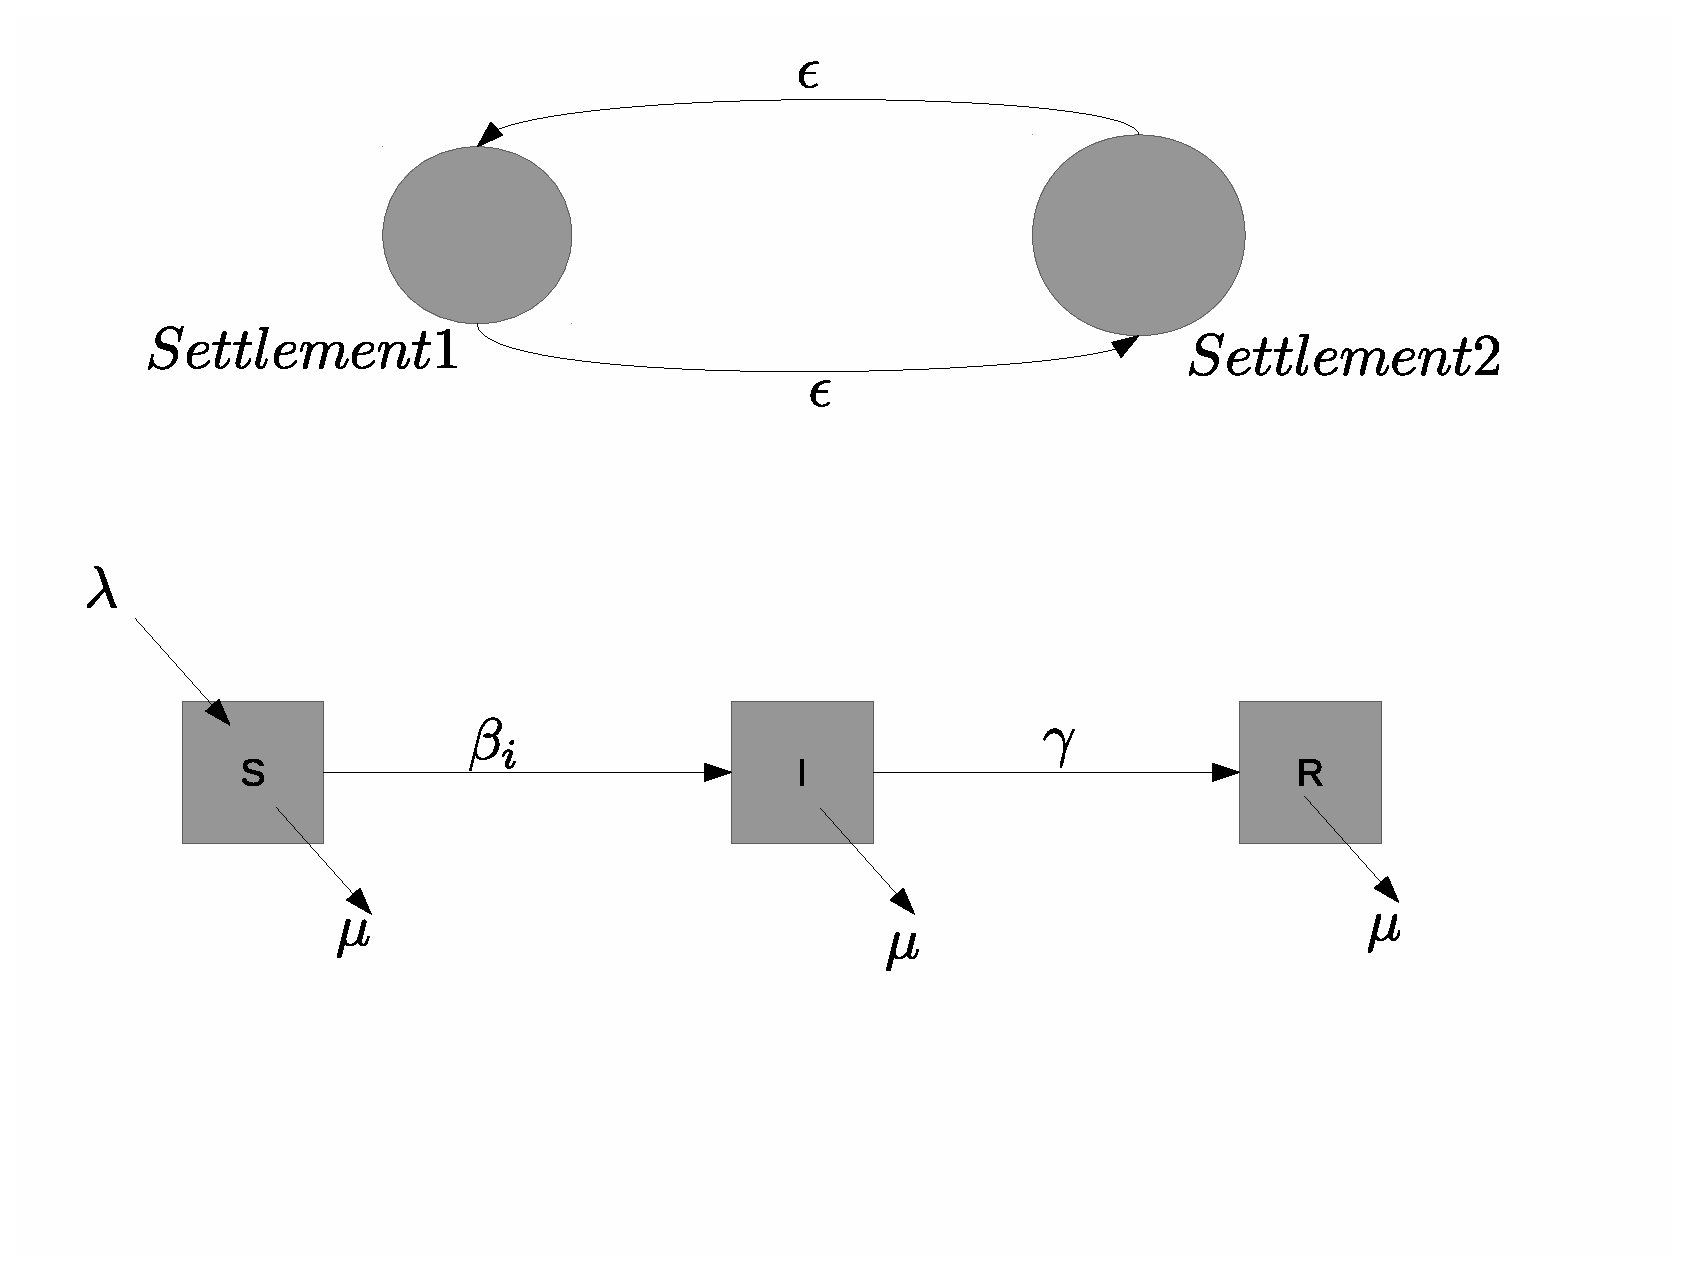
\includegraphics[width=\linewidth]{Figures_Tables/sir_im.eps}
  \caption{Each of the settlements contain this SIR compartments with $\epsilon$ as transfer rates between the settlements}
  \label{fig:SIR_des}
\end{figure}

The SIR model on two settlements is a modification of the conventional
SIR model accounting for the migration between the settlements.

%Equations
\begin{equation}
\begin{aligned}
\frac{dS_{1}}{dt} &= \lambda(S_{1}+I_{1}+R_{1}) -\mu  S_{1} - \beta_{1} S_{1}I_{1}  + \epsilon S_{2} -\epsilon S_{1} \\
\frac{dI_{1}}{dt} &= -\mu  I_{1} + \beta_{1} S_{1}I_{1}  + \epsilon I_{2} -\epsilon I_{1} -\gamma I_{1} \\
\frac{dR_{1}}{dt} &= -\mu  R_{1} +  \epsilon R_{2} -\epsilon R_{1} +\gamma I_{1} \\
\frac{dS_{2}}{dt} &=\lambda(S_{2}+I_{2}+R_{2}) -\mu  S_{2} - \beta_{2} S_{2}I_{2}  + \epsilon S_{1} -\epsilon S_{2} \\
\frac{dI_{2}}{dt} &= -\mu  I_{2} + \beta_{2} S_{2}I_{2}  + \epsilon I_{1} -\epsilon I_{2} -\gamma I_{2} \\
\frac{dR_{2}}{dt} &= -\mu  R_{2} +  \epsilon R_{1} -\epsilon R_{2} +\gamma I_{2} \\
\end{aligned}
\end{equation}
where $S_{i}$ is susceptible population of settlement i,$I_{i}$ is
infected population of settlement i,$R_{i}$ is recovered population of
settlement i,$\beta_{i}$ is transmission rate in settlement i(depends
upon the contact structure of settlement i), $\gamma$ is rate of
recovey, $\mu$ is the death rate, $\lambda$ is the birth rate and
$\epsilon$ the transfer rates between the settlements.

\iffalse
%Theoretical derivation
Similarly,there are several methods to estimate $R_{0}$ from a deterministic
model.                                                                                                           %cite the paper perspective on Ro.

We use Next generation operator method in this paper to calculate the
effective $R_{0}$ theoretically.
\fi

%Numerical derivation
There are several methods to estimate $R_{0}$ from
Epidemiological data. In this paper, we try to calculate $R_{0}$ from
intrinsic growth rate $r_{0}$. This growth rate is the rate at which                                             %References cite perspectives on r0
total number of infectives, $I$ grows in a susceptible population,
such that $\frac{dI}{dt}=r_{0}I$.Since we need epidemiological data to
calculate $r_{0}$ and subsequently $R_{0}$, Gillespie algorithm was                                                       %References cite Gillespie
used to stochastically simulate the model.                                                                          %(reference back to equations)
$r_{0}$, the intrinsic growth rate is estimated in the following way,
infection time series obtained from stochastic simulations were averaged
over 50 iterations to remove stochastic fluctuations, selecting only
simulations that lead to an epidemic outbreak in any of the
settlements.

The resulting averaged time series was then used to estimate $r_{0}$ by
applying regression procedure(at the initial part) to the logarithm of the
number of infected cases [$\log$(\#infected)] vs., time. To quantify the
quality of regression, we calculate $R^{2}$ the coefficient of
determination on the regression of the time series.$R^{2}$ is a
statistical measure of how close the data are to the fitted regression
line. $R^{2}$ ranges from 0 to 1 with 1 indicating exponential fit of
the number of infections vs., time.

We set $R^{2}_{cutoff}$ (here, $R^{2}_{cutoff}=0.75$) and select only
the slope of the fit whose $R^{2} > R^{2}_{cutoff}$ as an estimate of
$r_{0}$ and average them over 100 iterations to calculate the standard
deviation and mean of the estimated $r_{0}$, which will give us an
estimate on the range of variation of the estimated $r_{0}$. \par

$R_{0}$ is estimated from $r_{0}$ by using the relation                                           %Refrences cite how generation intervals shape....
between $R_{0}$ and $r_{0}$ with the assumption that the
generation interval distribution of the infected is exponential.                                             %Should we reason out why exponential?

Generation interval distribution is the probability distribution of
time from infection of an individual to infection of a secondary case
by that individual. The realtion between $R_{0}$ and $r_{0}$ is
established in \textit{(J. Wallinga and M. Lipsitch, 2006)}
\begin{equation}
R_{0}=\frac{1}{M(-r_{0})}
\end{equation}
where $M(z)$ is the moment generating
function of the generation interval distribution. Here, assuming
exponential distribution with mean $\frac{1}{\gamma}$ we find that(for
the derivation see supplimentary
material) $$R_{0}=1+\frac{r_{0}}{\gamma}$$ Using this relation we
estimate the effective $R_{0}$ at various transfer rates(see fig).                                               %Give the figure number for results
\subsection{SEIR model on 2 settlements}

%To add the figure of SEIR
\begin{figure}[h!]
  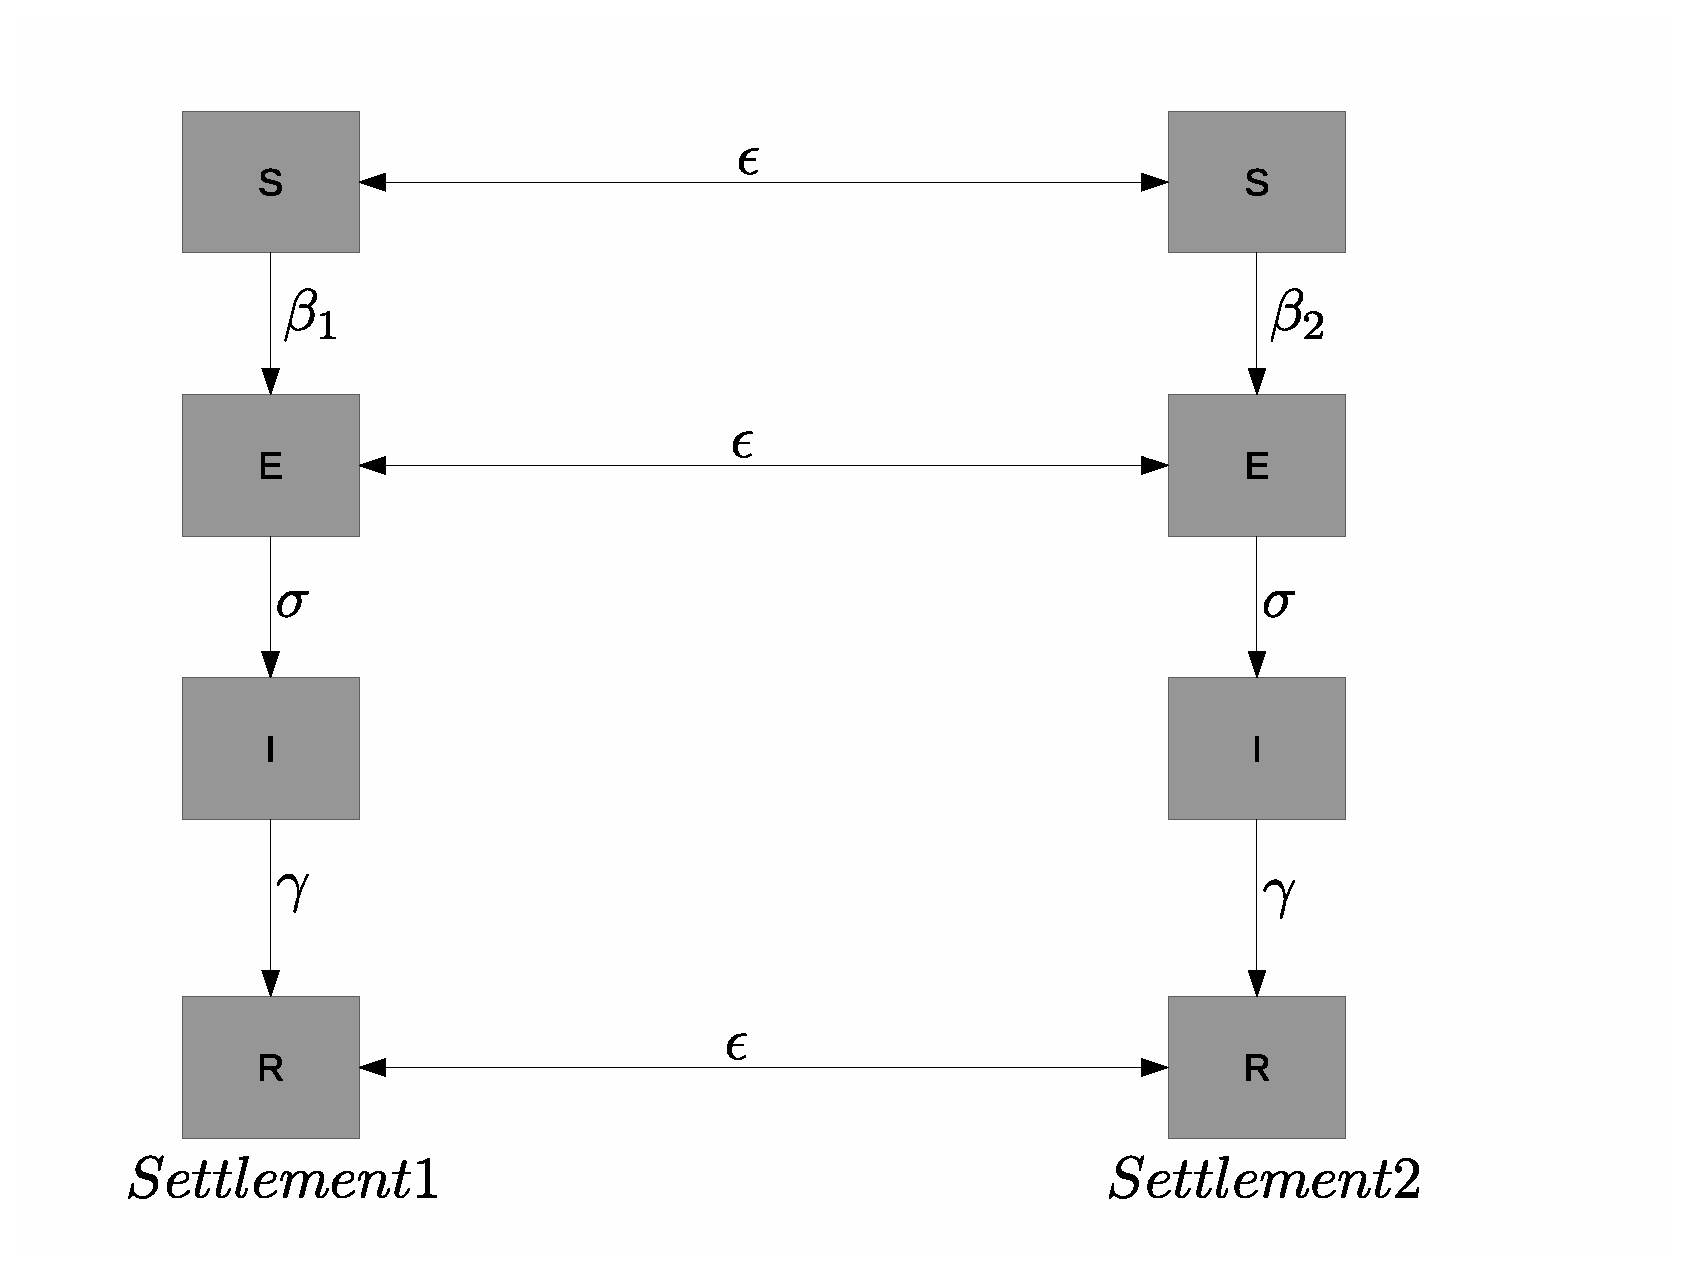
\includegraphics[width=\linewidth]{Figures_Tables/seir_im.eps}
   \caption{SEIR model}
  \label{fig:SIR_des}
\end{figure}

In this SEIR model infected individuals are restricted to migrate,
which is a fair assumption to make since diseases can render an
infected individual incapable of migration.

%Equations
\begin{equation}
  \begin{aligned}
\textbf{Equations} \\
\frac{dS_{1}}{dt} &=\lambda(S_{1}+E_{1}+I_{1}+R_{1}) -\mu  S_{1} - \beta_{1} S_{1}I_{1}  + \epsilon S_{2} -\epsilon S_{1} \\
\frac{dE_{1}}{dt} &= -\mu  E_{1} + \beta_{1} S_{1}I_{1}  + \epsilon E_{2} -\epsilon E_{1} -\sigma  E_{1} \\
\frac{dI_{1}}{dt} &= \sigma E_{1} -\gamma I_{1} -\mu I_{1} \\
\frac{dR_{1}}{dt} &= -\mu  R_{1} +  \epsilon R_{2} -\epsilon R_{1} +\gamma I_{1} \\
\frac{dS_{2}}{dt} &=\lambda(S_{2}+E_{2}+I_{2}+R_{2}) -\mu  S_{2} - \beta_{2} S_{2}I_{2}  + \epsilon S_{1} -\epsilon S_{2} \\
\frac{dE_{2}}{dt} &= -\mu  E_{2} + \beta_{2} S_{2}I_{2}  + \epsilon E_{1} -\epsilon E_{2} -\sigma  E_{2} \\
\frac{dI_{2}}{dt} &= \sigma E_{2} -\gamma I_{2} -\mu I_{2} \\
\frac{dR_{2}}{dt} &= -\mu  R_{2} +  \epsilon R_{1} -\epsilon R_{2} +\gamma I_{2} \\
  \end{aligned}
\end{equation}
where $\sigma$ denotes the rate of becoming infected after being exposed and all other variables denote same as in SIR.

%Numerical Derivation
Same method of calculating $R_{0}$ from intrinsic growth rate $r_{0}$
as in SIR model was applied. Here we assume generation interval
distribution as convolution of two exponential distributions with mean  
$\frac{1}{\sigma}$ and $\frac{1}{\gamma}$. From eq() we find the relation                                           %To fill up the equation number
between $r_{0}$ and $R_{0}$ to be
\begin{equation}
  R_{0}=(1+\frac{r_{0}}{\sigma})(1+\frac{r_{0}}{\gamma})
\end{equation}
Using the above relation we estimate effective $R_{0}$ of the
settlements at various transfer rates, see fig()                                                                             % To add figure number

\section*{Results}

\subsection{SIR Model}
Individual $R_{0}$ of the settlements were calculated using
theoritical formula $\frac{\beta_{i}N_{i}}{\gamma}$. We observe that
as transfer rates between the settlement increase the effective
$R_{0}$ of the system tends toward the mean of the individual $R_{0}$
of the settlements, in all three cases irrespective of where the
infection arises the effective $R_{0}$ tends towards the mean.
\begin{figure}[H]
  \hspace*{-2cm}
  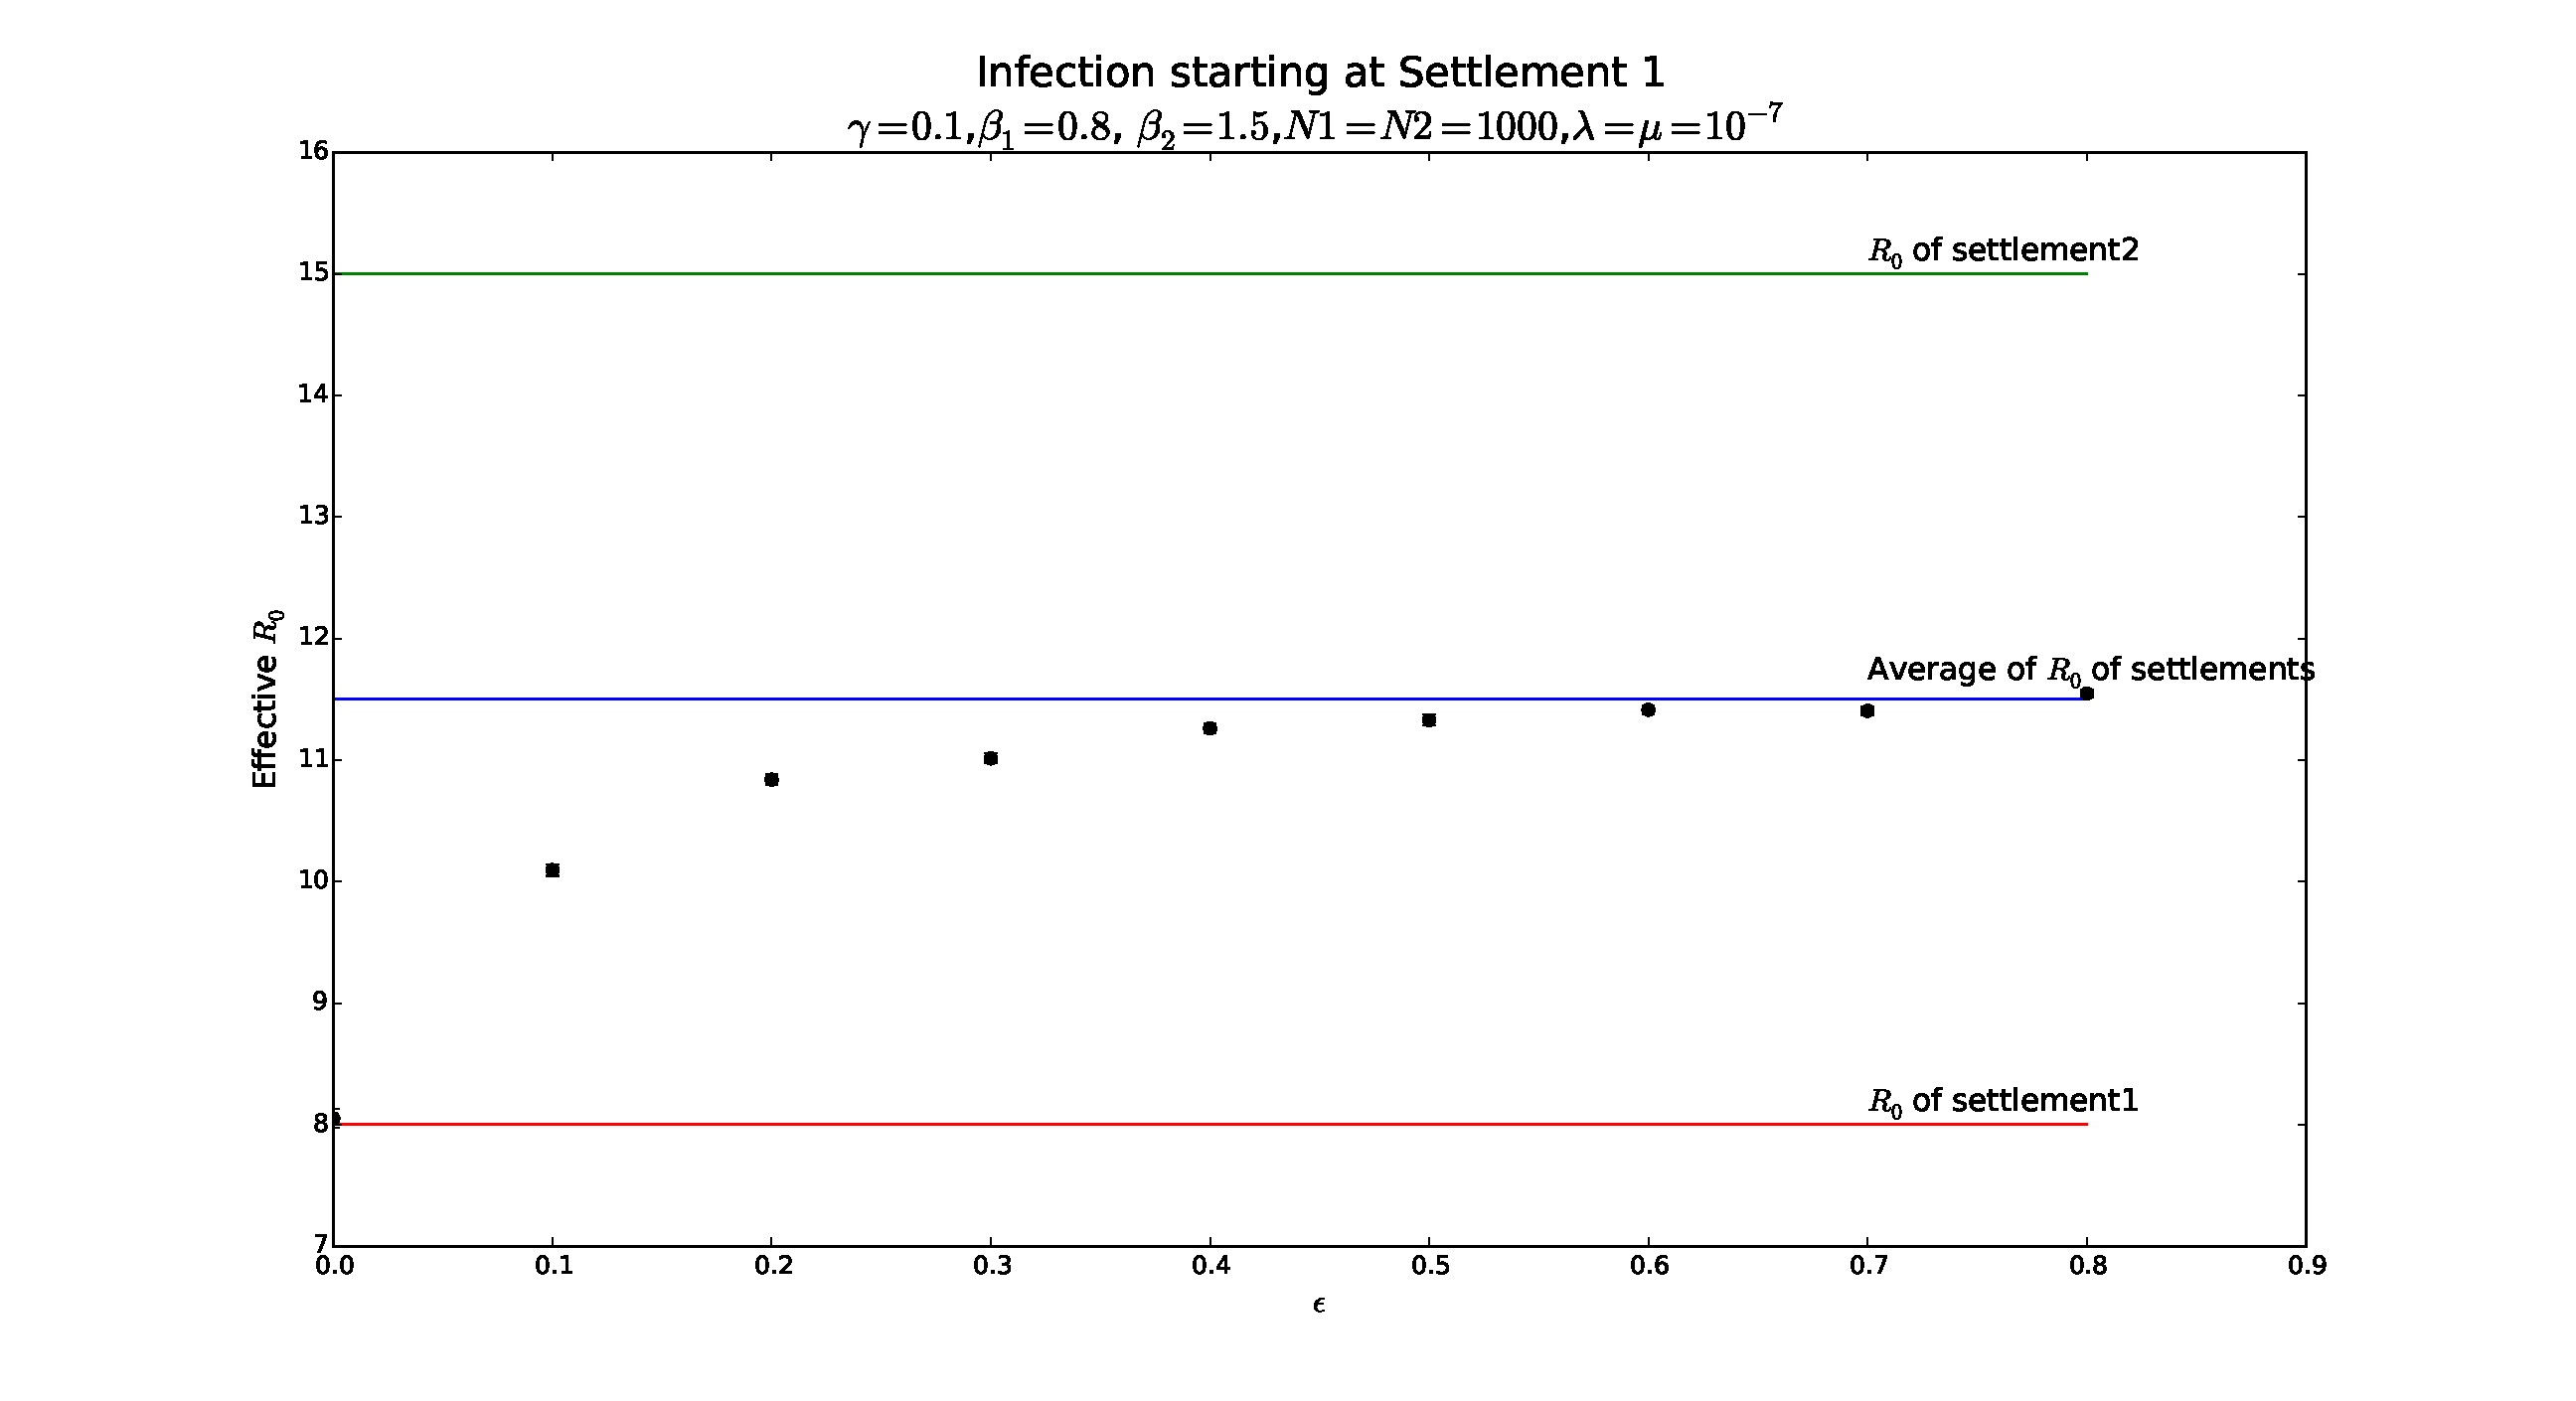
\includegraphics[scale=0.4]{Figures_Tables/sir_1inf.eps}
  \hspace*{-2cm} 
  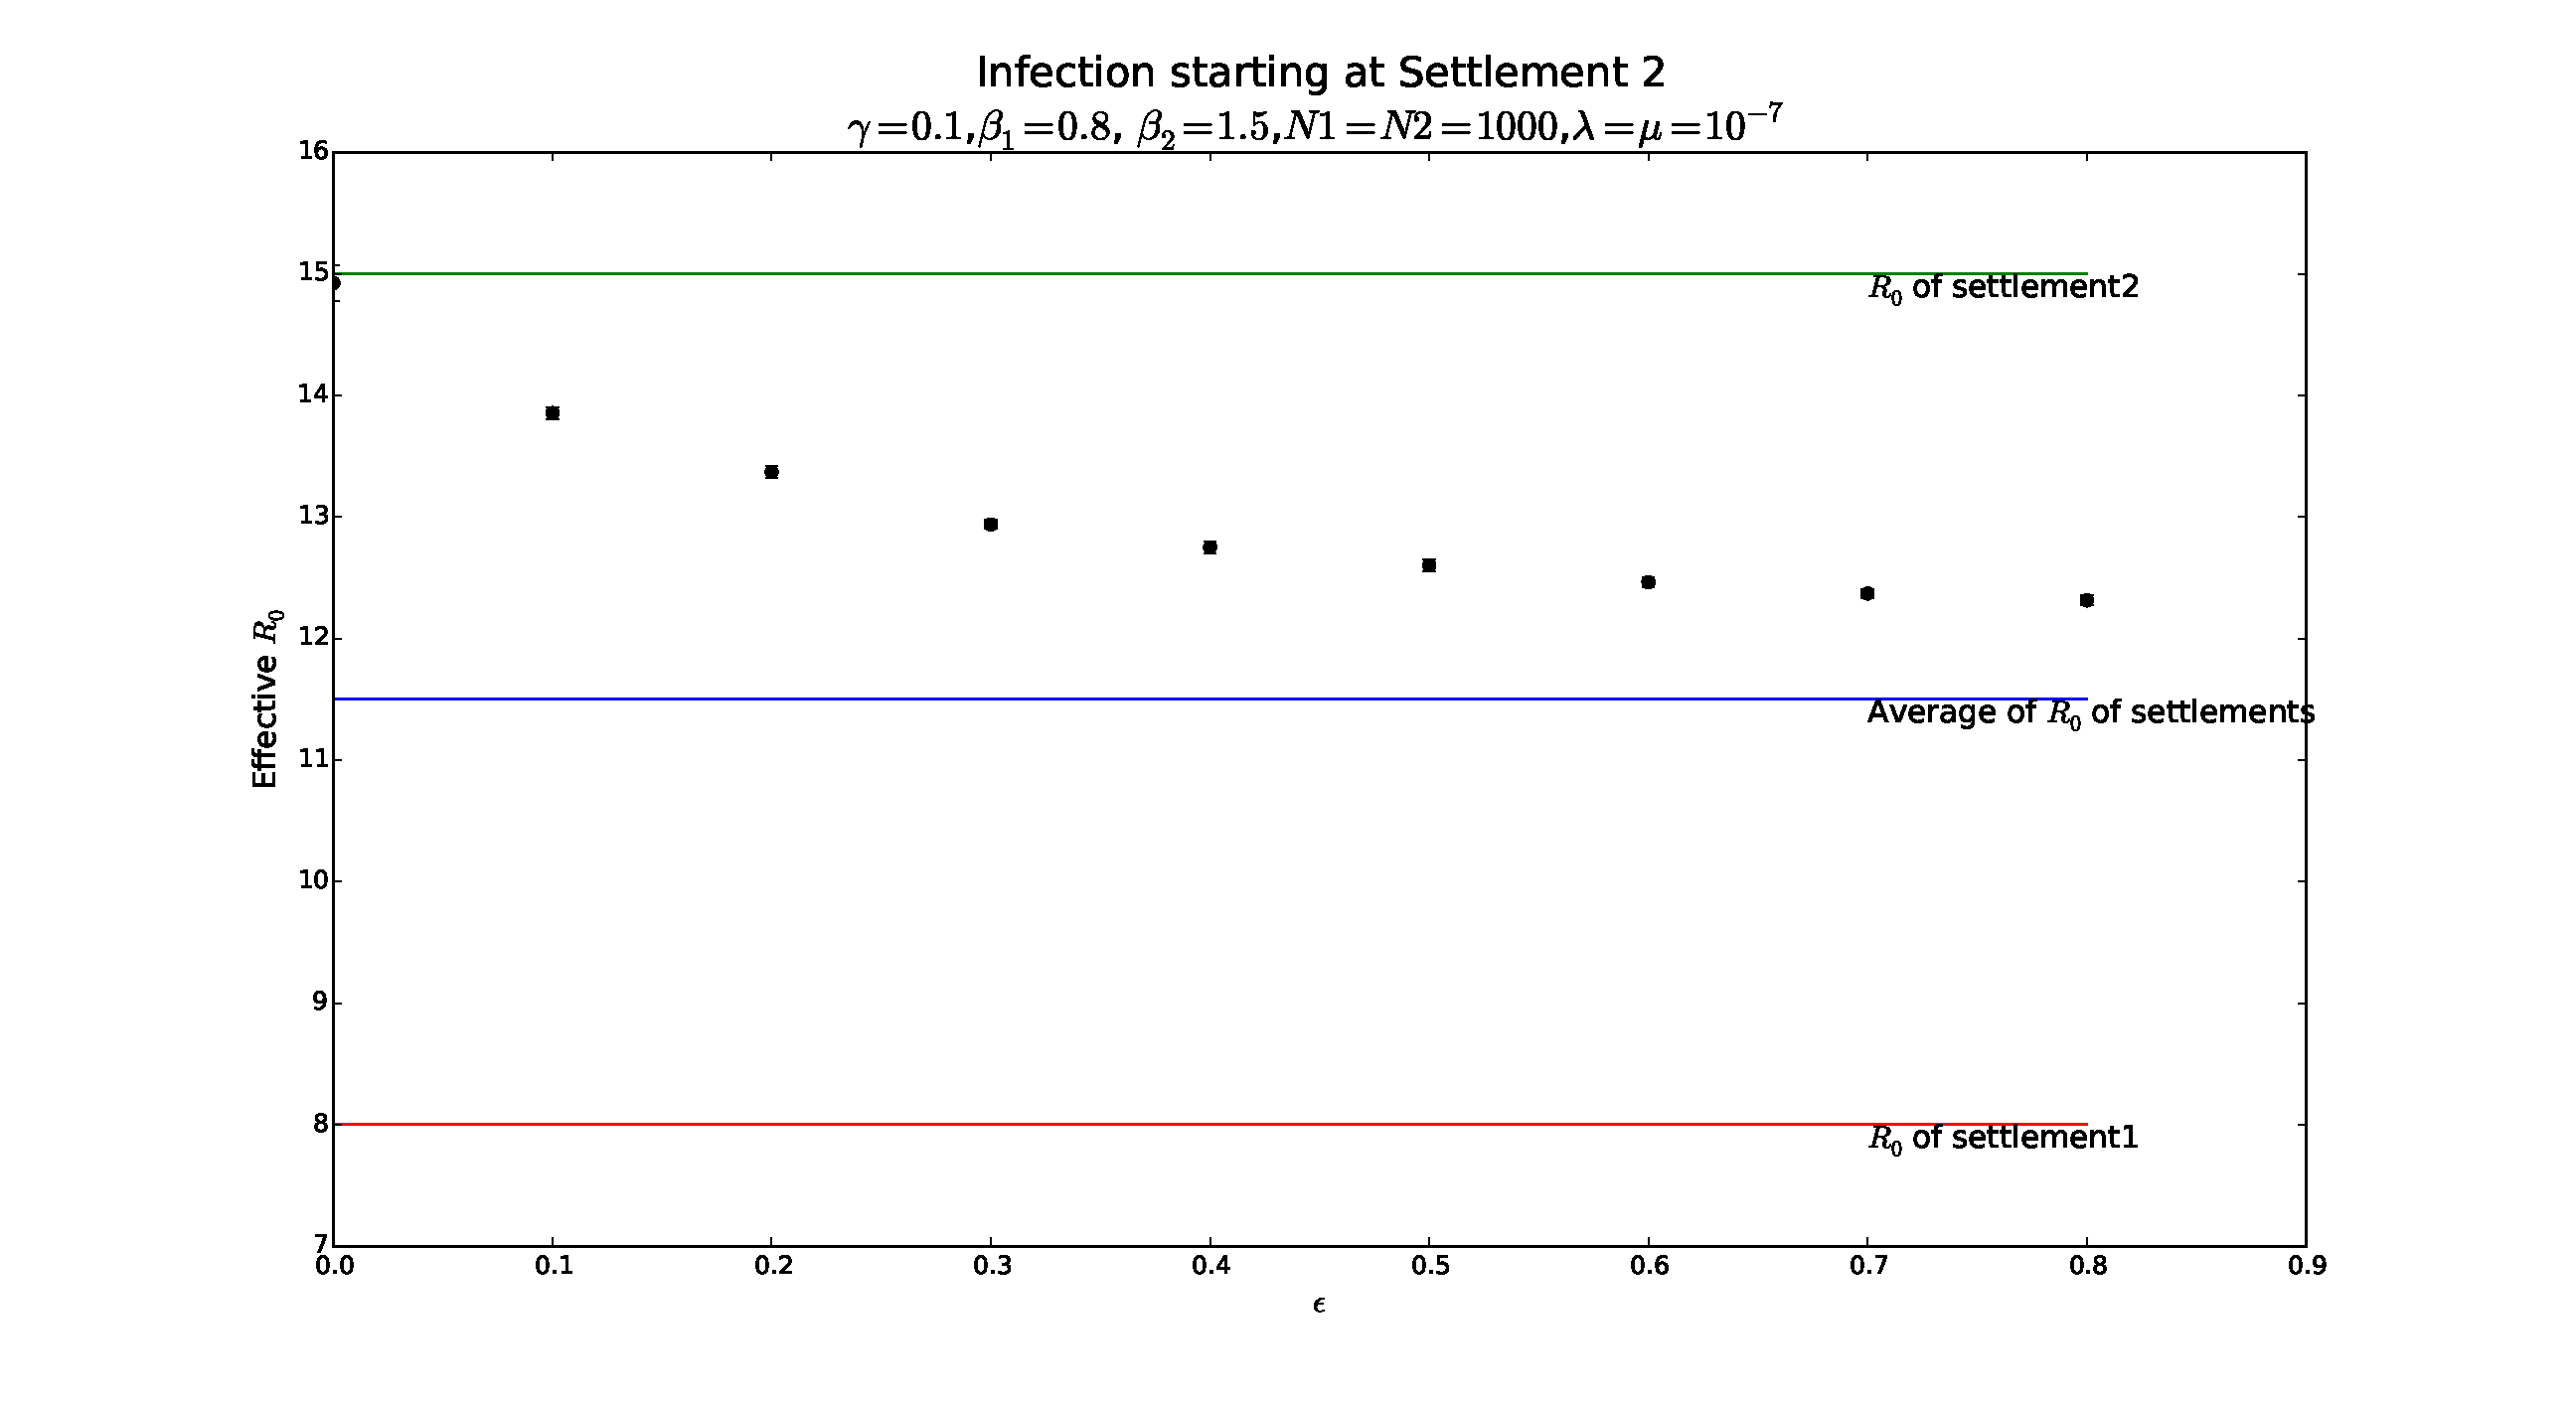
\includegraphics[scale=0.4]{Figures_Tables/sir_2inf.eps}
\end{figure}
\begin{figure}[H]
\hspace*{-2cm}
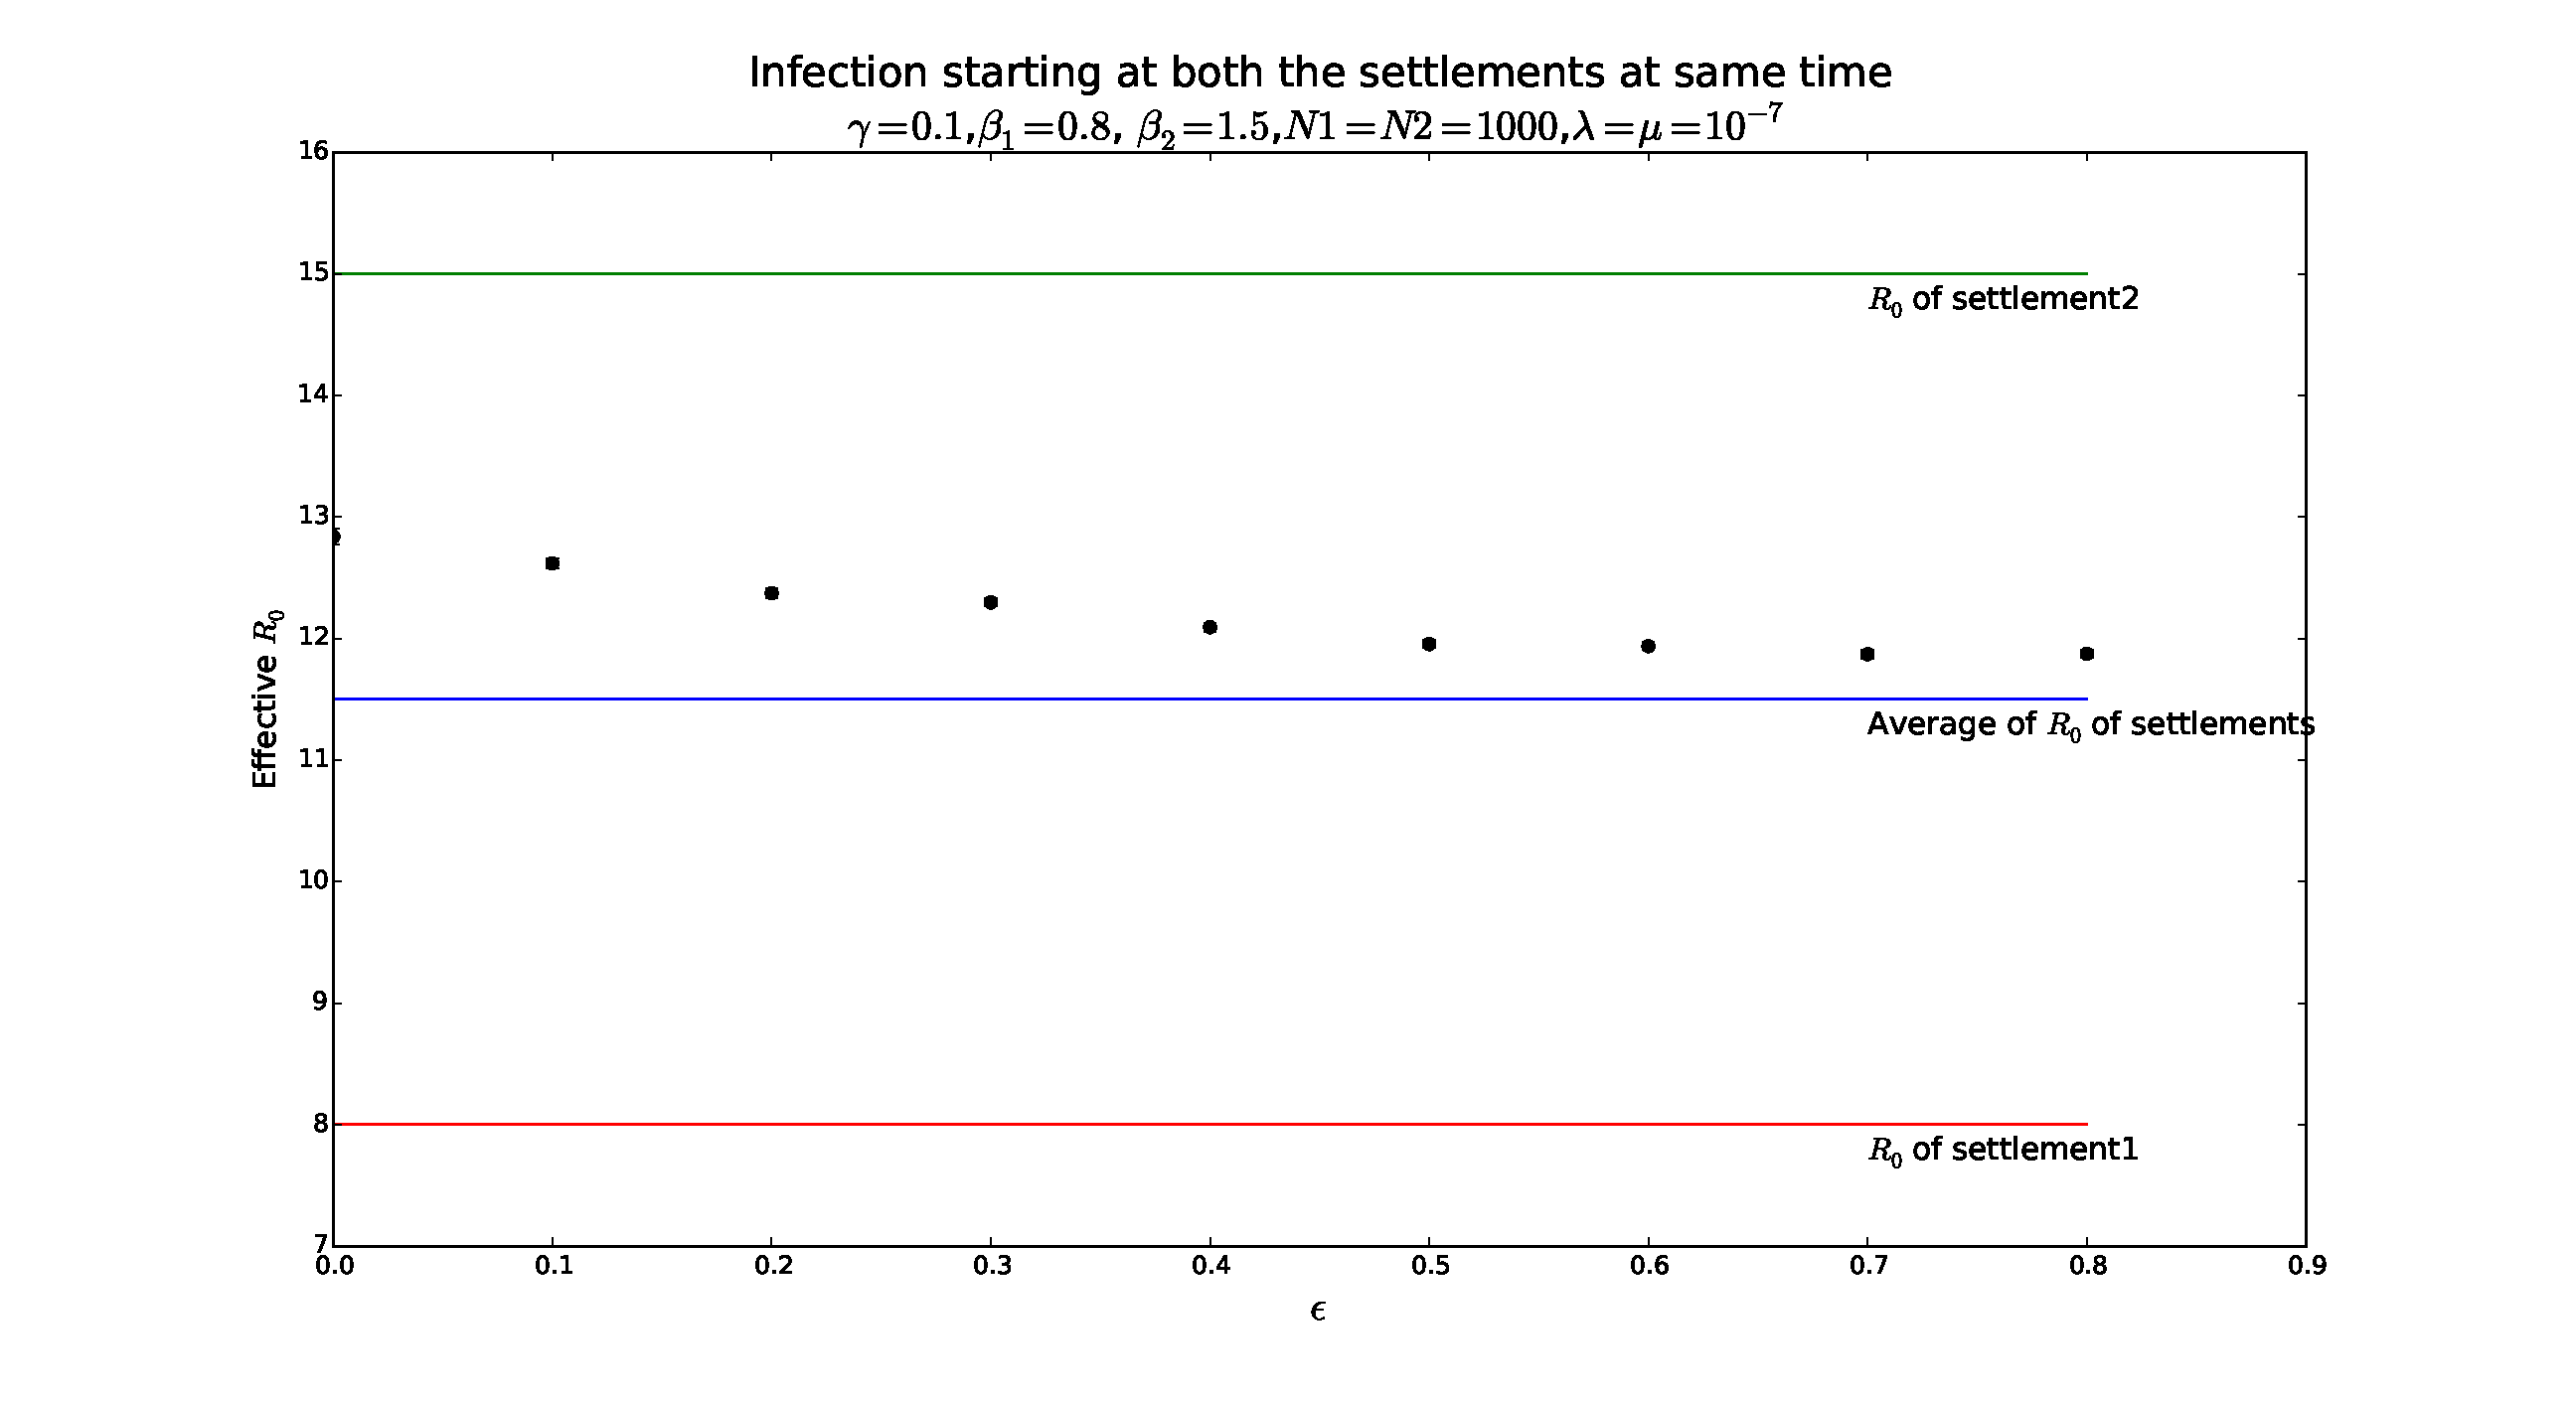
\includegraphics[scale=0.4]{Figures_Tables/sir_12inf.eps}
\end{figure}


\subsection{SEIR model}
Individual $R_{0}$ of the settlements were calculated using
theoritical formula $\frac{\beta_{i} N_{i}
  \sigma}{(\gamma+\mu)(\mu+\sigma)}$. We observe similar pattern as in
SIR model, effective $R_{0}$ of the system converges to the mean of the
individual $R_{0}$ of the settlements.
\begin{figure}[H]
  \hspace*{-2cm}
  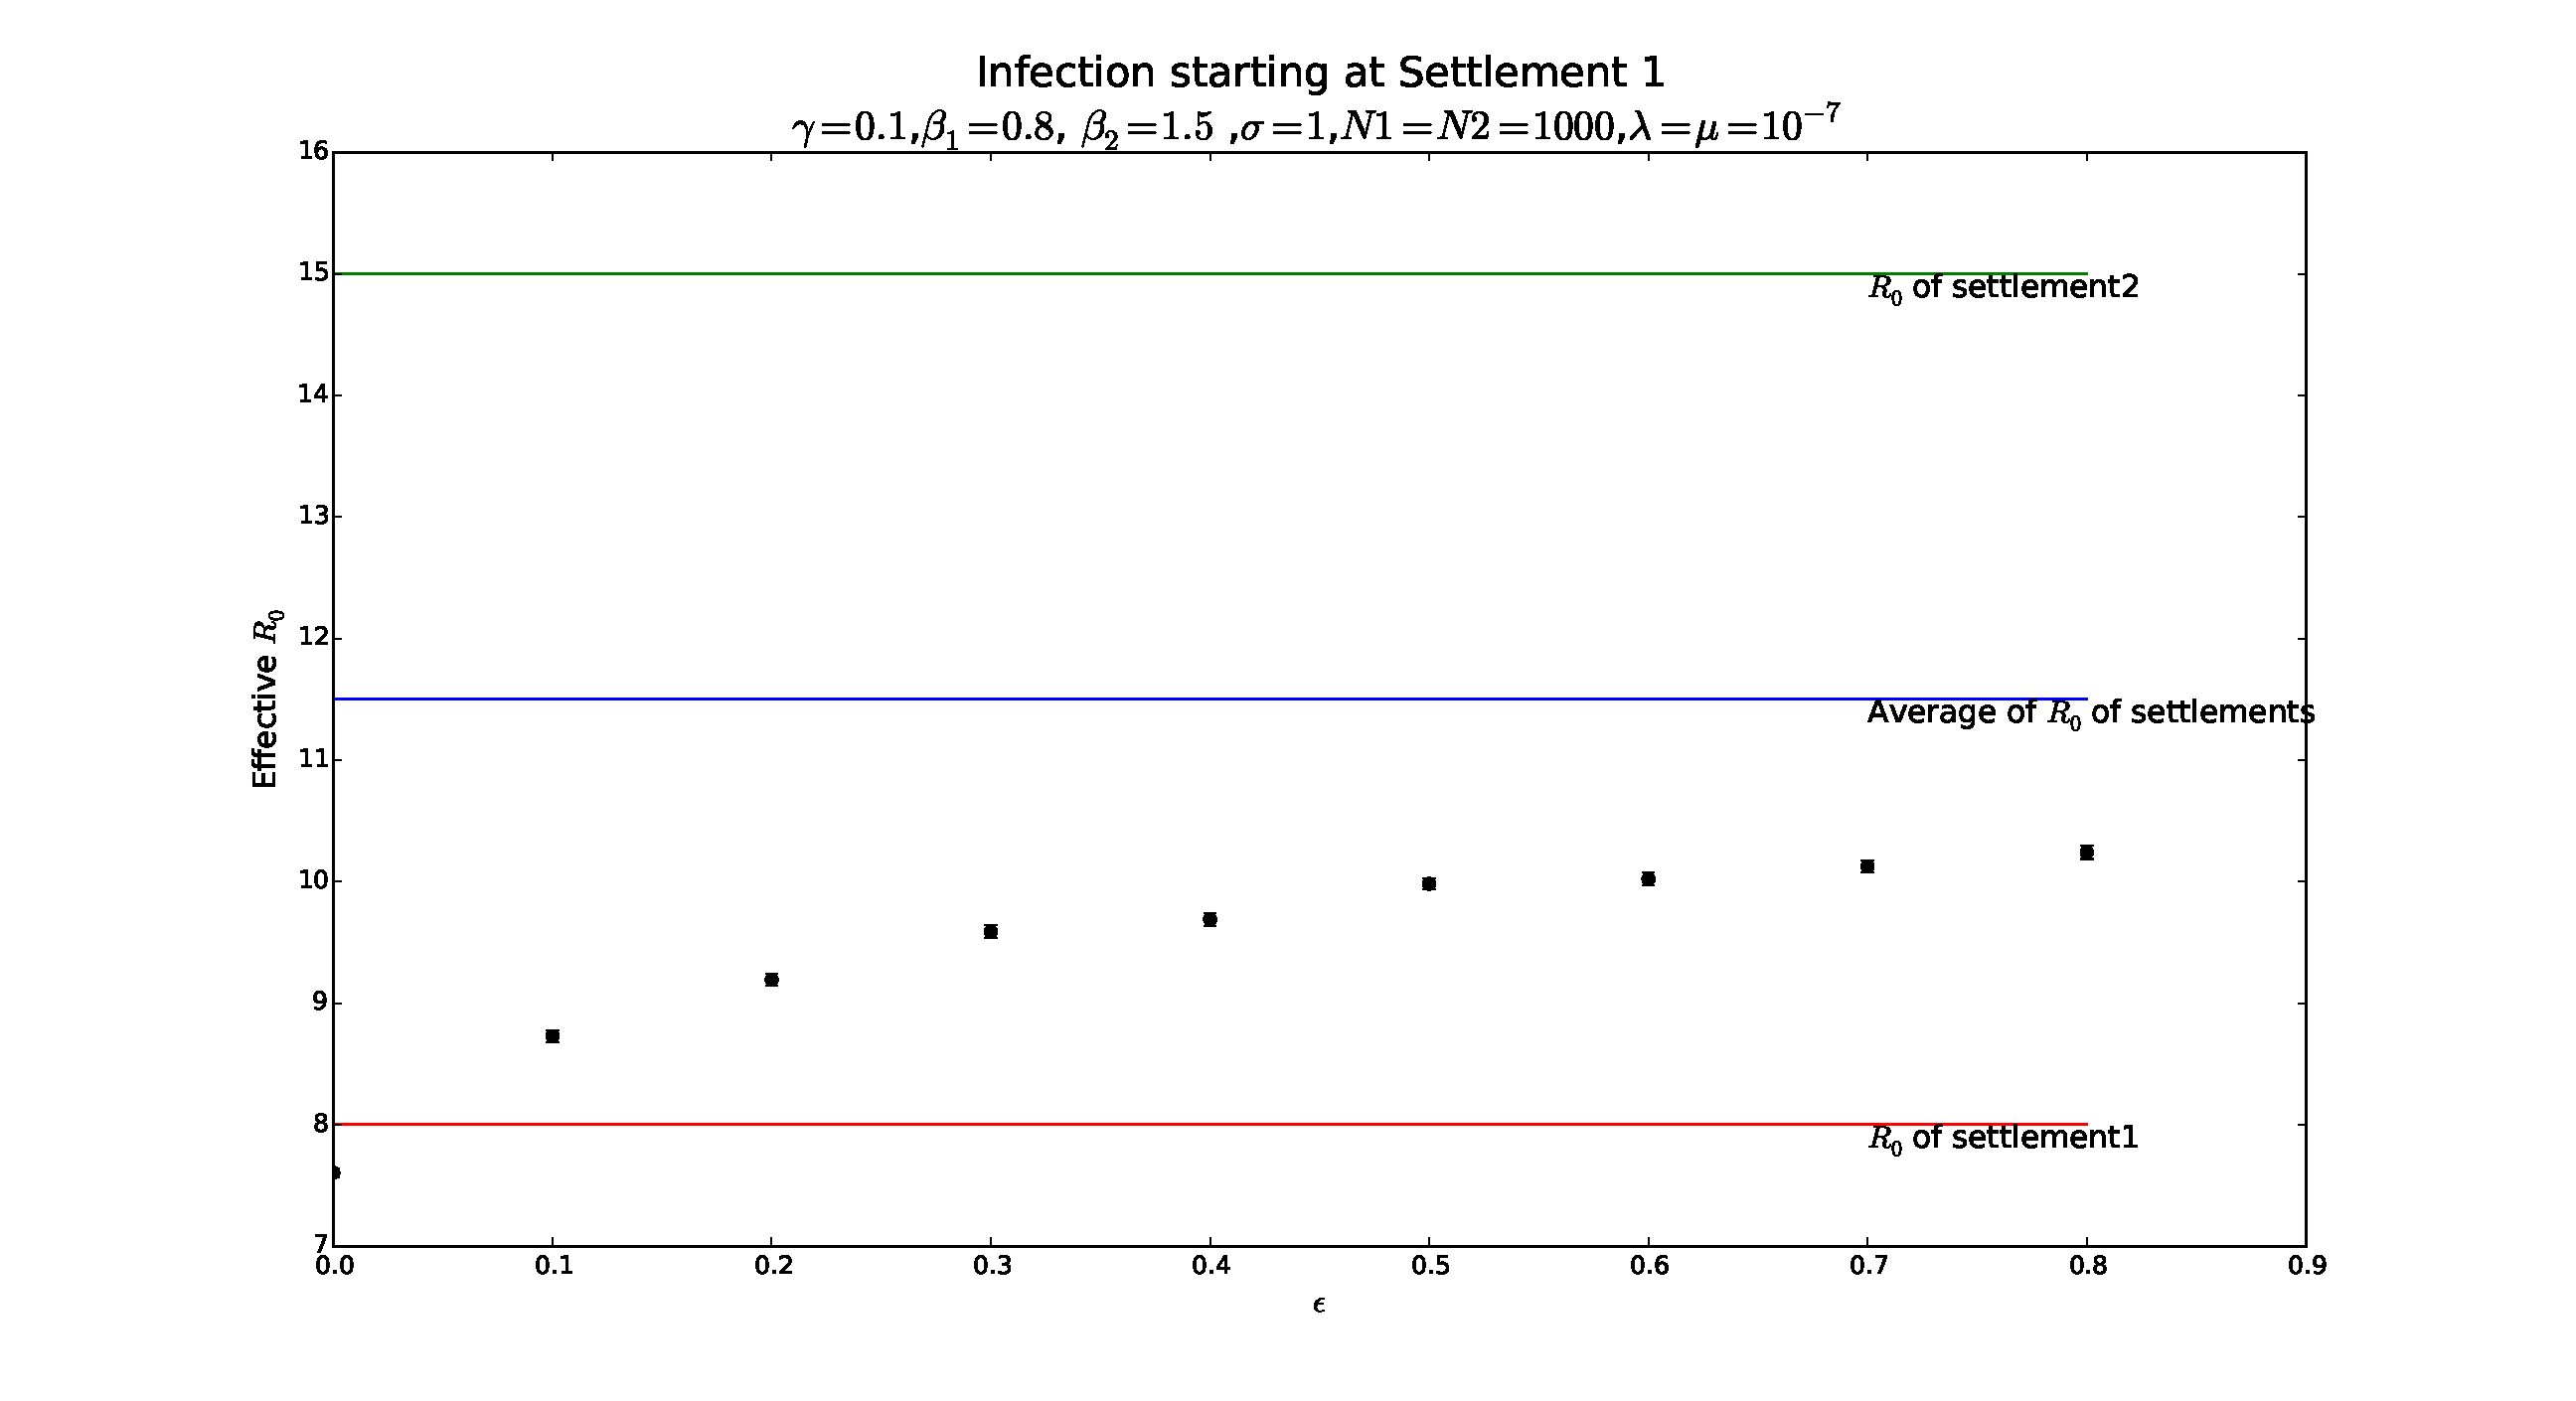
\includegraphics[scale=0.4]{Figures_Tables/seir_1inf.eps}
  \hspace*{-2cm} 
  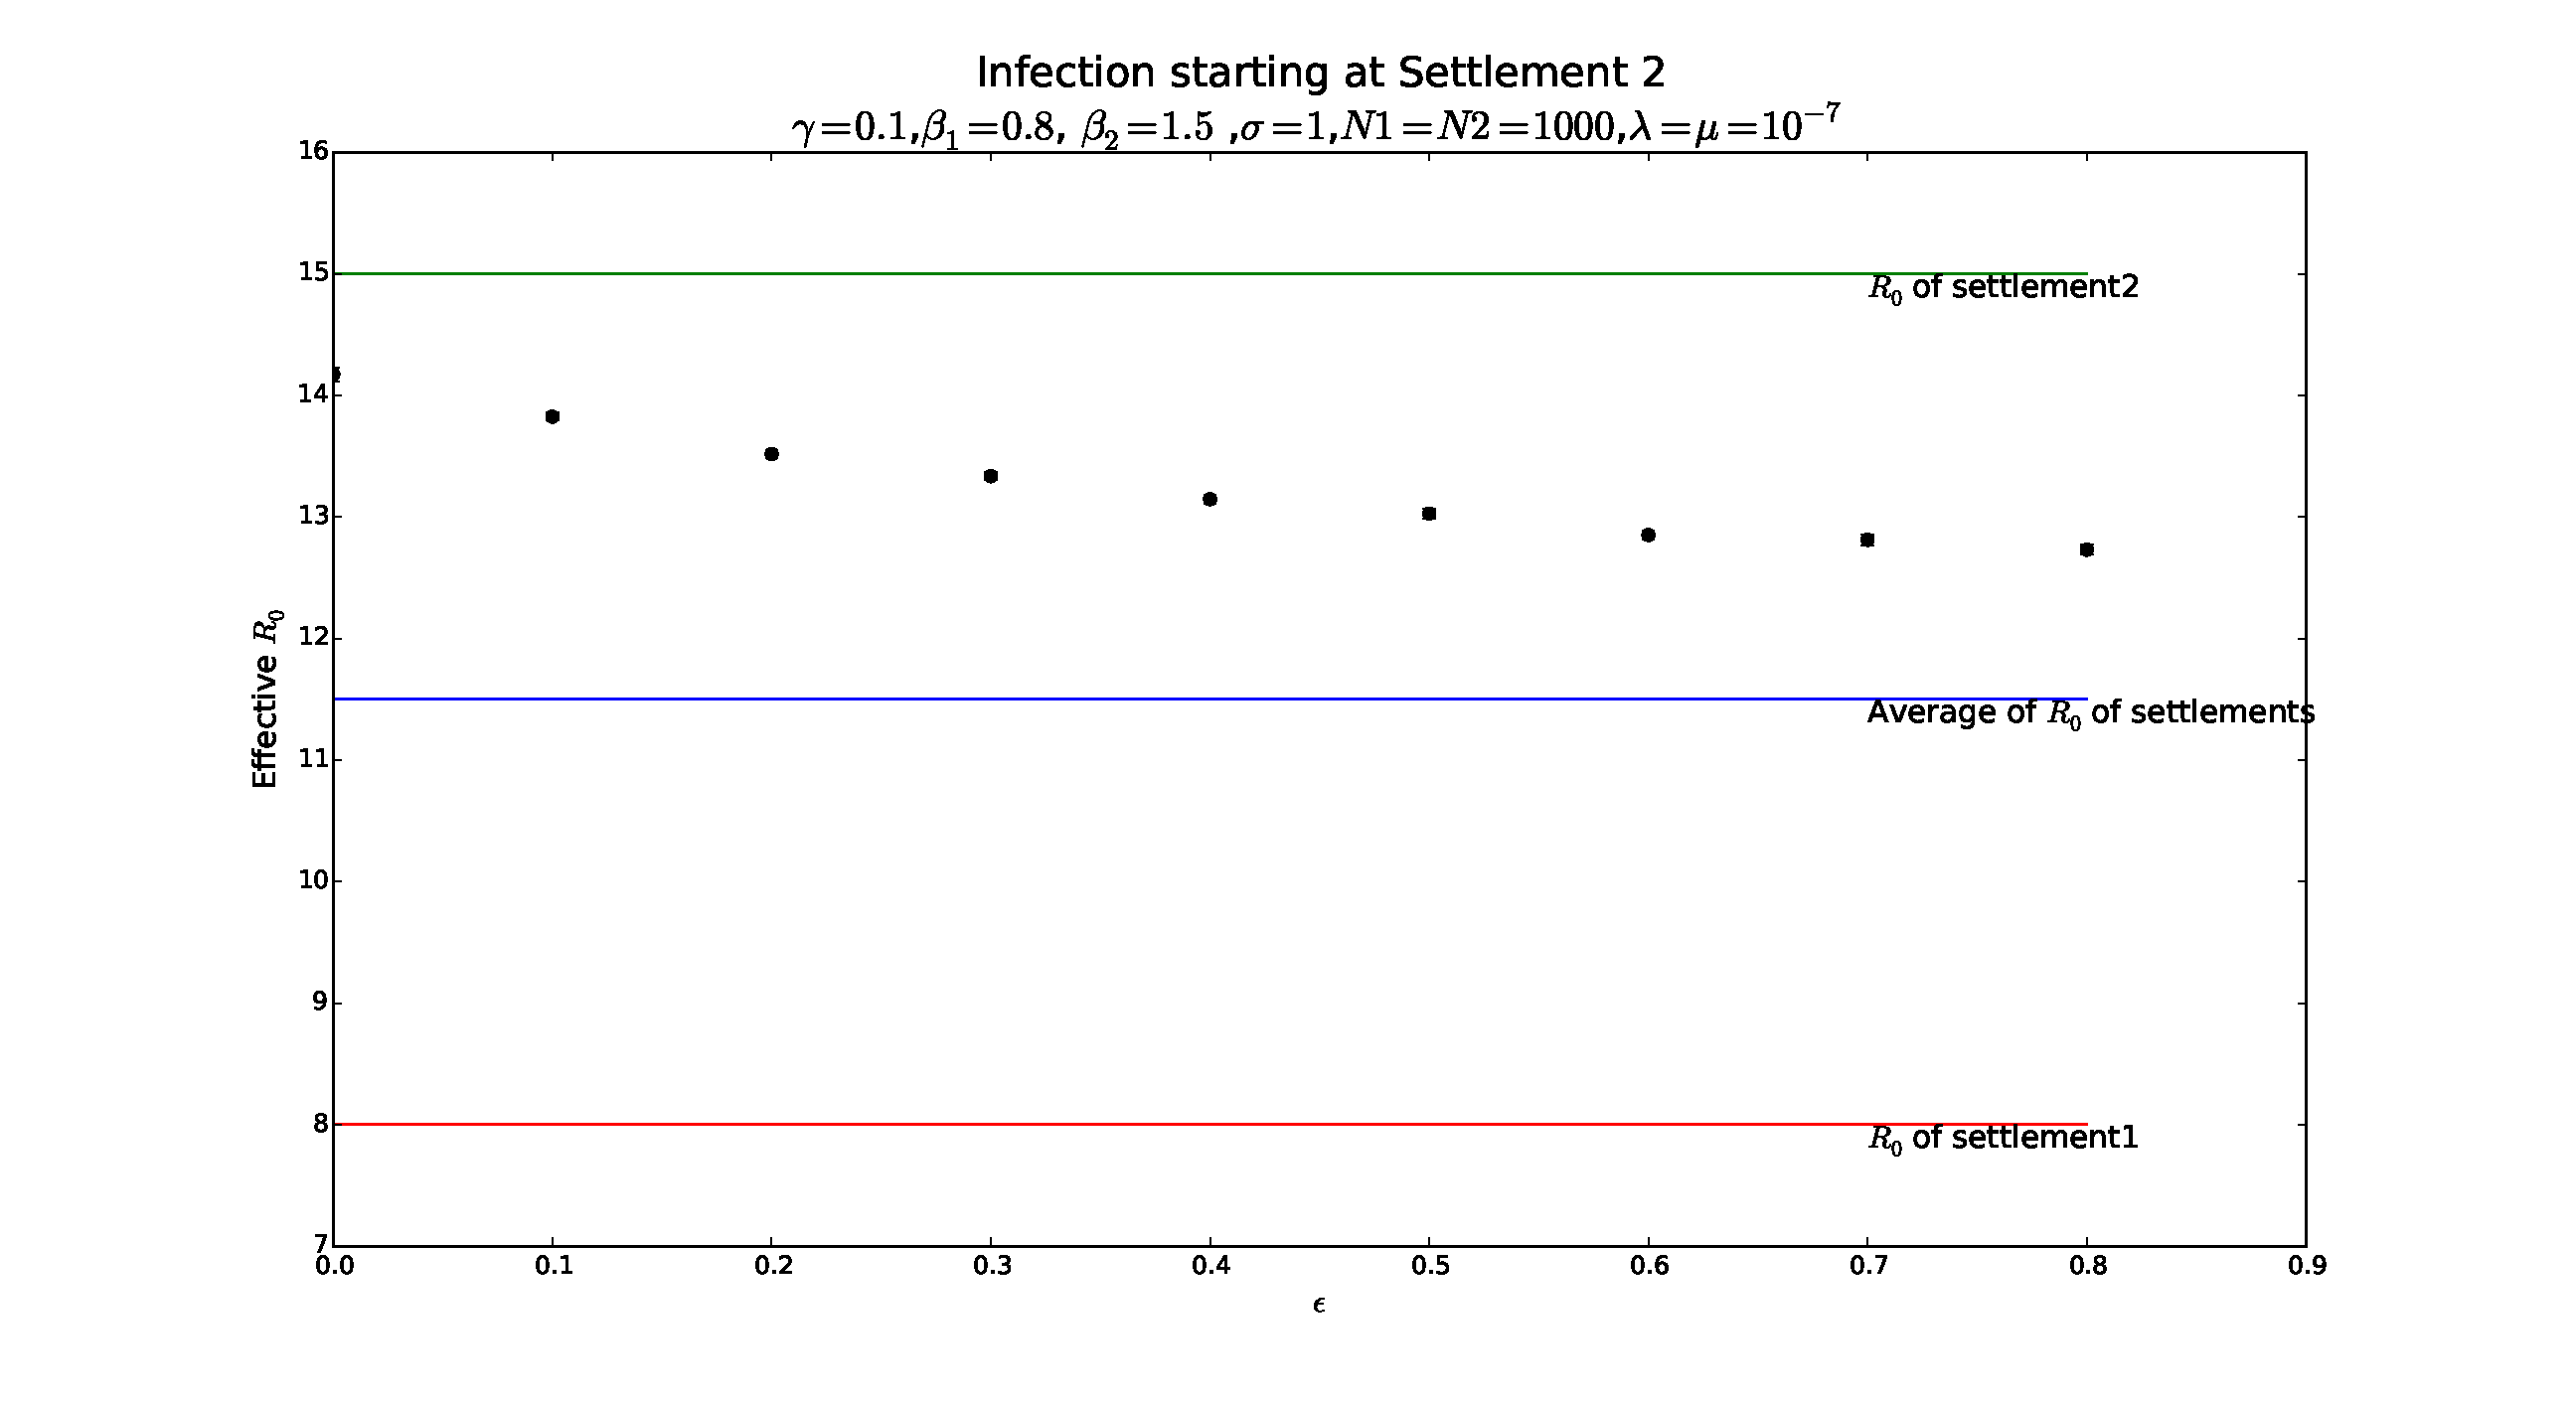
\includegraphics[scale=0.4]{Figures_Tables/seir_2inf.eps}
\end{figure}
\begin{figure}[H]
\hspace*{-2cm}
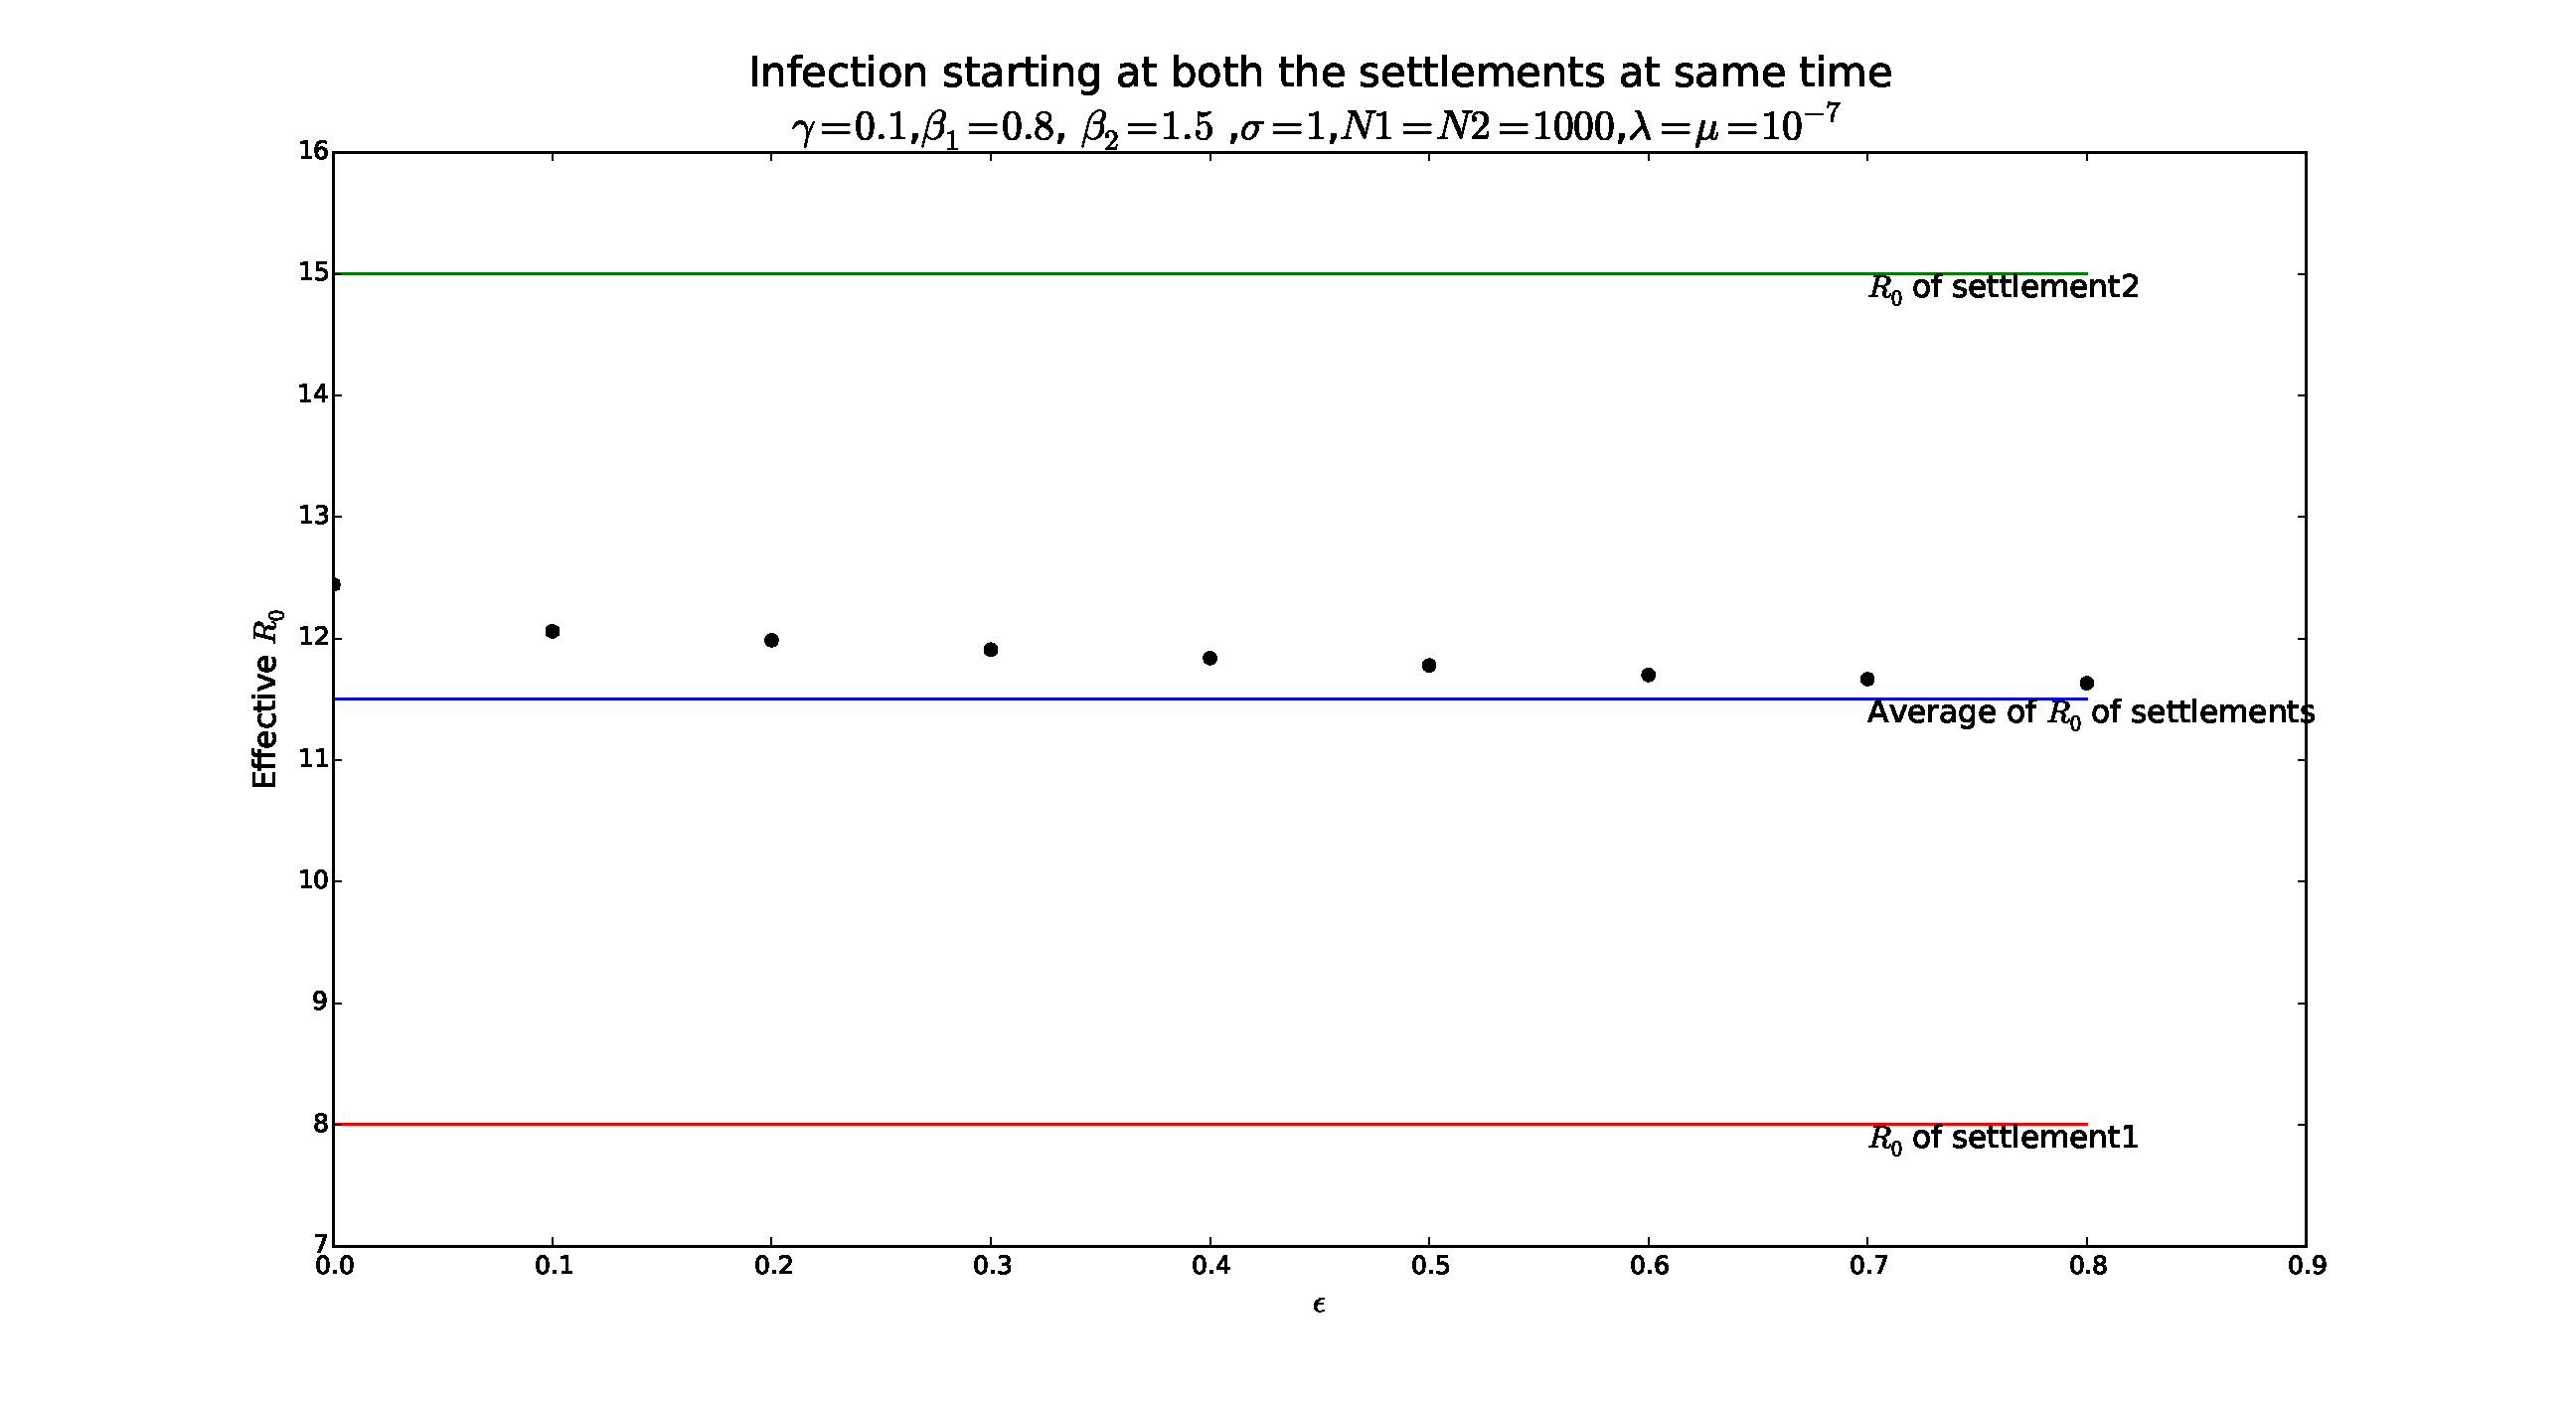
\includegraphics[scale=0.4]{Figures_Tables/seir_21inf.eps}
\end{figure}
\section*{Conclusion}
One may easily underestimate or overestimate the $R_{0}$ of the
system, if they don't consider the rate of movement between the
settlements. These rate of movements can be approximated by transport
networks such as airlines,railway connectivity and other such
transport modes. One can easily underestimate the $R_{0}$ if the
disease first devolops in a settlement which has less contact rate
$\beta$. Simillary overestimate if the disease devolopes in a
settlement which has a higher contanct rate. So one should keep in
mind that transport rates between settlements plays an important role
in estimation of effective $R_{0}$ of a country or a system.

\end{document}
